\documentclass[11pt]{article}
\usepackage[margin=1in]{geometry}
\usepackage{amsmath,amssymb,array,booktabs,hyperref,xurl,pdfpages}
\hypersetup{hidelinks,pdftitle={Supplement on the Farey induction}}
\title{Supplement on the Farey induction\\[4pt]\large Integer superharmonic matrices on the $F$-lattice}
\author{}\date{}
\newcommand{\Z}{\mathbb Z}
\setlength{\emergencystretch}{2em}
\Urlmuskip=0mu plus 2mu
\begin{document}
\maketitle
This supplement accompanies Sections 6, 8 and 9 of the paper. The two base-case calculations are reproduced in full at the end. For mixed words the three numbered parts below give the statements used in Section 9, the order of their proofs, and the locations of the geometric estimates. Each part names an archive delivered with this supplement. All paths in a part are relative to that archive unless stated otherwise.

\section*{I. Ranks of the standard and alternate fields}
\noindent\emph{Source:} \path{standard-and-alternate-fields.zip}. The account in \path{plane-fields.md} assembles the induction; \path{chronology/ABSTRACT_ALL_WORD_CHRONOLOGY.md} is its copy inside the archive.

Fix an even proper child with numerator and denominator $n,d$, and write its odd parent as $N/D$. Set $\epsilon=Nd-Dn$, $U=(d,n)$, $V=(n-d,n+d)$, $\sigma=2\epsilon(D,N)$ and $v=\epsilon(N-D,N+D)$. These shifts are in the physical lattice. The transverse coordinate is $t(x,y)=nx-dy$. On the standard polygon the construction controls the differences between $F$ and its two signed short translates. It also carries the two zero levels $2-d-n$ for the even standard and $1-d-n$ on even physical parity for the odd standard, in their respective transverse coordinates. The pure formulas initialize these levels and both signs of the ranks. The empty word has its own actual initial data. See \path{chronology/PURE_COMPLETE_INTERFACE_AUDIT.md}.

\paragraph{How the new standard gets its rank.}
For each sign the cut estimates provide two integer quantities $P,J$ which do not increase along the forced interior edges. The second is the rounded signed difference in that orientation. Their increments under the period translations are constant. For positive integer weights $a,c$, put $K=aP+cJ$. If a forbidden set is bounded below in $K$, at a minimal site each continuing interior step stays at the same values of $P$ and $J$. The interior directed graph modulo the two periods has no directed cycle, hence such continuation reaches a free boundary site. Normalize that site by translating the entire forbidden set. For the specified pair of values of $P,J$ there are only finitely many possible boundary sites, by independence of their two period increments. The boundary comparisons in \path{escape/ALL_SLOPE_STEP.md} give, from each one, either a site earlier in the elimination order for the same pair or a site where both quantities are no larger and one is strictly smaller. The latter contradicts minimality; the former runs out of sites. At a black site the argument permits either input which belongs to the forbidden set.

One endpoint value is particularly sensitive to the choice of period representative. Write the odd parent's longitudinal coordinate as $s_p(x,y)=(D+N)x+(D-N)y$. Then
\[
 s_p(V)=(D+N)(n-d)+(D-N)(n+d)=2(Dn-Nd)=-2\epsilon .
\]
Thus the terminal value in these two orientations is $2N-2\epsilon$ when the initial value is zero. The reflected negative-orientation endpoints are $-2,2N$. The construction uses this increment in the vertical boundary case. The earlier ranks and zero levels used to justify the interior arrows and boundary choices are in \path{chronology/B2_INDEPENDENT_PRERANK_AUDIT.md} and \path{canonical/wave1close/W1_CONSTRUCTOR.md}. The corrected endpoint computation is incorporated in \path{canonical/strong_bulk/STRONG_PRICE_AND_ALTERNATE_STEP.md}.

Here is the passage from escape to a rank. Under the above estimates there is a uniform finite time $h$ to force the grade below its initial value, for either black input, using the chosen white strategy. Otherwise finite branching gives an infinite surviving set in one of the lower-bounded half-spaces just excluded. Taking the maximum over a period cell gives a common $h$. Let $d_0$ bound the absolute grade change of an individual edge. Concatenating successful segments of length at most $h$, a play stopped at time $t$ obeys
\[
                 t+hK(z_t)\le hK(z_0)+h+h^2d_0 .
\]
Indeed each completed segment lowers the grade by at least one, and the final partial segment can increase it by at most $h d_0$. Set $R_0=hK$ and
\[
 R_{j+1}(x)=\max\{hK(x),1+\mathcal T R_j(x)\},\qquad
 \mathcal T R(x)=
 \begin{cases}
 \min_{y\in I(x)}R(y),&\Delta F(x)=0,\\
 \max_{y\in I(x)}R(y),&\Delta F(x)=-1 .
 \end{cases}
\]
The displayed bound, applied also to intermediate stopping times, bounds the increasing integer functions $R_j-hK$ uniformly. They are periodic, so this sequence stabilizes on the finite cell. The limiting inequalities provide a decreasing white input and two decreasing black inputs on the whole plane. The detailed uniform escape and stopping-time arguments are in \path{escape/weighted_rank_audit/WEIGHTED_FORT_AND_BELLMAN_RANK.md}.

\paragraph{Why the threshold minimum propagates.}
For the two prescribed fields $A,B$ write $\Phi=A-B$ and $m_k=\min(A,B+k)$. Their geometric comparisons give $|\Phi(y)-\Phi(x)|\le1$ at both inputs. The signed $A$ choices make $\Phi$ nonincreasing, and the signed $B$ choices make it nondecreasing. At a strict winner, that field still wins weakly on the whole incoming star. At a tie, a black sheet wins weakly on both of its inputs. If both sheets are white, the increments of $\Phi$ on the two inputs sum to zero and have size at most one, so the tie loses at most one unit under the Laplacian. These cases give $\Delta m_k\in\{-1,0\}$.

Use $-|\Phi-k|$ as the first rank coordinate, and the winner's strict rank as the second. Use $A$'s rank on the tie band. At a strict winner its chosen edges either increase the distance to $k$ or preserve it and strictly decrease that sheet's rank. At a black tie retain both inputs. An edge leaving the band strictly decreases the first coordinate. Any edge staying on it which must be retained is an $A$ edge: at a black $A$ both are chosen; at a white $A$ with an increment requiring the other edge to be rejected, monotonicity forces selection of the tie. At a white tie both increments vanish, so $A$'s chosen input works. Interchanging the roles on the tie gives the other signed choice. This proves recurrence at every integer threshold on the plane. On the tie band the signed rank with zero period increment gives the stronger finite-period burning order used at the next step. The all-input bounds and the exclusions for the actual two parents are in \path{canonical/strong_bulk/STRONG_PRICE_AND_ALTERNATE_STEP.md}, \path{canonical/strong_bulk/TWO_RANK_RAW_PHI_AUDIT.md} and \path{canonical/strong_bulk/CHAIN_BAND_AUDIT.md}. The earlier parent identification is in \path{canonical/cut_origin/ACTUAL_CHAIN_CONJUGACY_ALL_CREATORS.md}. The complete midpoint calculation used for the alternate is in Section 9 of the paper and in \path{canonical/strong_bulk/alternate_midpoint/MIDPOINT_LEMMA.md}.

\section*{II. Ordered tile construction}
\noindent\emph{Source:} \path{ordered-tile-construction.zip} and the accompanying \path{finite-tile-identification.md}. Number the six source positions as in \path{Code/src/offsets.jl}, from 1 to 6. The additional position 7 is the older alternate in the ordinary alternate construction. The actual order in which the positioned functions are normalized is
\[
\begin{array}{l|l}
\text{output}&\text{insertion order}\\ \hline
\text{standard odd, ordinary or corrected}&1,2,5,6,3,4\\
\text{standard even, ordinary or corrected}&1,3,4,2,5,6\\
\text{alternate odd, ordinary}&1,7,3,4,2,5,6\\
\text{alternate even, ordinary}&1,7,2,5,3,4,6\\
\text{alternate, corrected, either type}&1,3,4,5,6,2
\end{array}
\]
For a short correction of index $k\ge0$ there are $k+1$ copies of the first standard, one copy of the second at the join, and $2k+1$ copies of the old alternate. The long correction has $2k+2$ copies of the alternate. Both the actual earlier tiles and the place at which each was created enter its displacement. All sites of these pieces are retained.

Each insertion uses three estimates on one fixed target. The incoming height in the right additive normalization equals the target on all new sites, is at least the target on previously assigned sites, and is equal there at a genuine contact. These assertions apply in the integer coordinates of the actual earlier domain. For a correction using the last saved digit $1$, one must compare against the \emph{minimum} of the two targets. For example, let $Z=2a+R$ be the earlier birth, $A=Z-a$, $v=V_A$, $g=F_Z$ and $b_A=(n_A,-d_A)$ for $A=(d_A,n_A)$. In the first orientation put $P(u)=g(u)-g(u+v)+b_A\cdot u$ and $D(u)=g(u)-g(u-2A)$. For $p=P(u-v)-c_A$, where $c_A$ fixes the side normalization, and $d_0=D(u-v)$, the required right value is $\min(0,p-d_0)$. The common lower bound is $-2$ and $p=d_0=-2$ is excluded. The proof of this joint exclusion uses the longitudinal position in the actual birth polygon. A bound $d_0\ge-1$ throughout the larger window would fail. Both signs and the short and long occurrences, including the ordinary limiting placement, are checked in \path{recognition/prefix/saved1_true_birth_correction/PROPER_SAVED1_REPAIR.md} and its consumer comparison in the same directory.

For literal ancestors the four endpoint cases are the reciprocal and near-one families in each of the two phases. The first alternate insertion at the reciprocal right endpoint is computed in \path{recognition/prefix/PURE3_ENDPOINT_ORDERED_LONG_EXTENSION.md}. Its two values one unit above the old standard are retained at the old standard's height. The dual four-site endpoint is treated in \path{recognition/prefix/endpoint_G1_G2/pure2_four_site/DUAL_R0_ORDERED_G3_MERGES_CLOSED.md}. The six ordinary sources and the seventh source of an ordinary alternate are checked in \path{recognition/prefix/unc_final_review/UNC_ALL_ENDPOINT_WIRING_AUDIT.md}. To identify an odd alternate with its rounded global field on its \emph{own} domain, use \path{recognition/prefix/CURRENT_ODD_ALTERNATE_D_GUARD.md}. Its transverse bounds in the even companion's chart are $3-T\le t\le d+n-1$ on the current support. This gives the three-value interval for the height difference used in the minimum representation of the rounded field. Section 3 of \path{finite-tile-identification.md} gives the period increments and distinctness calculation, including the translated standard used in the reflected odd orientation.

\section*{III. Coverage by each finite tile}
\noindent\emph{Source:} \path{period-coverage.zip} and the accompanying \path{native-coverage.md}. The induction carries the assertion $D+L'(n,d)=\Z^2$ for the occupied domain $D$ of each of the four earlier tiles. In applying it to a standard one obtains the occupied inner region by removing all representatives outside the permissible grade interval. For an alternate one obtains a point on the actual row when its possible lift is unique. The outstanding narrow strips are covered by tracked finite source rows. Thus one may use the true earlier native sites in the new polygon at a specified grade. Coverage of a bounding polygon alone would not imply this assertion.

The literal initializers, including the root and pure runs, are proved in the file headed \emph{Literal initializers}. For the ordinary standards use the six-source propagation in \path{F_LATTICE_FULL_ORDINARY_STANDARD_COVER_PROPAGATION_20261119.zip}. For the alternates and for the corrected standards, the table in Section 9 gives the digit and the length of the correction. The transition table in \path{native-coverage.md} gives the corresponding proofs for the two signs, the two saved histories and the pure endpoints. In particular a corrected earlier standard already exists, with its own coverage, when its saved copy is used. The case with last saved digit $3$ in a run of twos uses \path{F_LATTICE_W1_SHORT_SAVED3_CORRECTED_SEED_CHRONOLOGY_ERRATUM_20261120.md}. The reciprocal comparisons at a fixed depth first establish the ordinary standards and the direct two-run cases from older domains. Their reciprocal uses then have a previously established current case. This gives a separate proof of coverage for every output. Agreement of the translated heights is supplied by part II.

\section*{Base cases}
The following two papers contain the explicit period overlaps, rank corrections and directions of decreasing input for all denominators. The first treats the odd denominators $d\ge3$. The second treats the doubled staircases at even $d\ge4$, their reciprocal partners and the checkerboard correction. The change of variables in \path{base/BASE-DUALITY-PROOF.md} identifies the domains, values and physical placement of both reciprocal families at odd $d$. The editable sources and algebraic tables are in \path{base/}.
\clearpage
\pdfbookmark[1]{Odd denominators: standard and alternate}{odd-base}
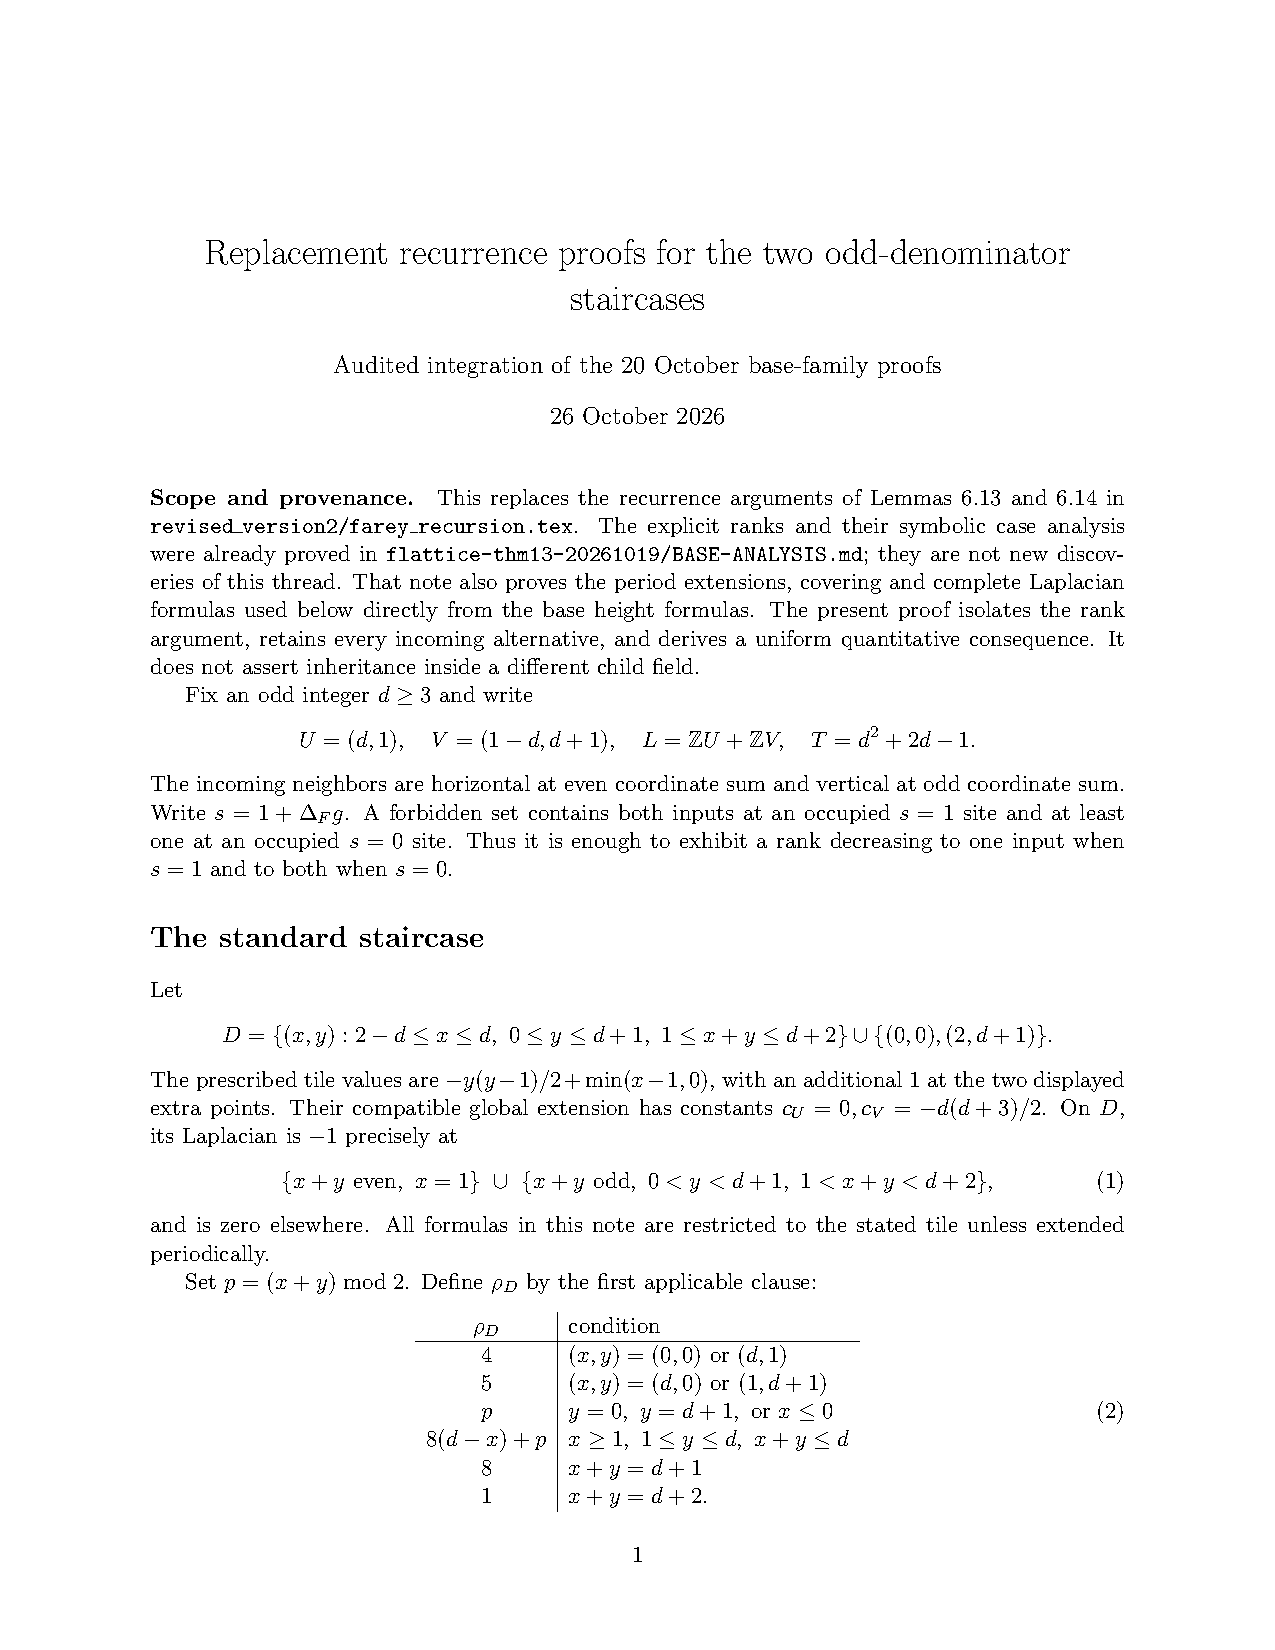
\includepdf[pages=-,pagecommand={}]{base/staircase_recurrence_replacement.pdf}
\pdfbookmark[1]{Even denominators and the physical rotation}{even-base}
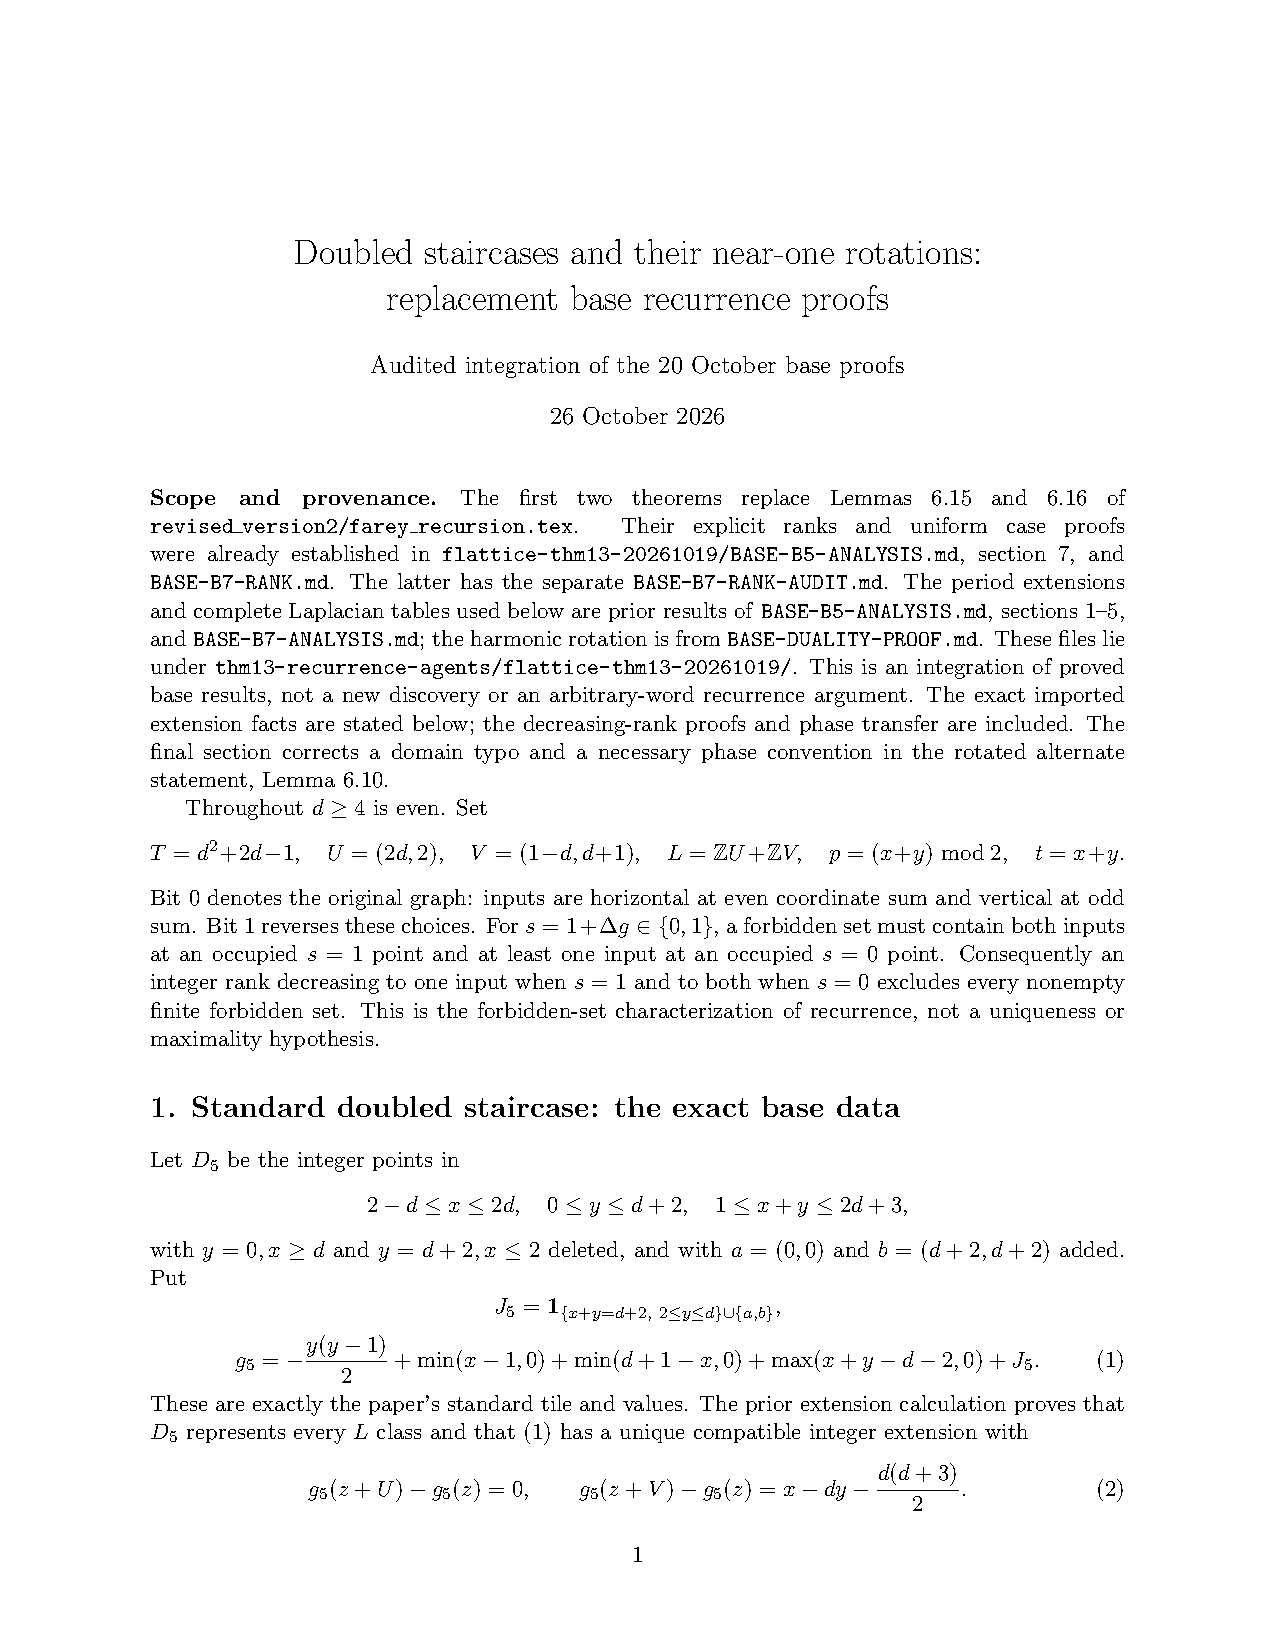
\includepdf[pages=-,pagecommand={}]{base/near_one_base_recurrence_replacement.pdf}
\end{document}
